
\documentclass[11pt]{article}
\usepackage[utf8]{inputenc}
\usepackage{geometry}
\usepackage{amsmath}
\usepackage{amsfonts}
\usepackage{amssymb}
\usepackage{graphicx}


\newgeometry{left=3cm, right=2.5cm, top=2.5cm, bottom=2.5cm}


\newcommand{\abbrlabel}[1]{\makebox[3cm][l]{\textbf{#1}\ \dotfill}}
\newenvironment{abbreviations}{\begin{list}{}{\renewcommand{\makelabel}{\abbrlabel}}}{\end{list}}

\title{\begin{Large}
\textbf{Sensor Network For Air Pollution Monitoring}
\end{Large}\\ Master's Thesis Proposal}
\author{Ashlin Saju}

\date{}
\begin{document}
\maketitle
\newpage
\tableofcontents
\newpage

\section{Introduction}

Air pollution is a matter of serious concern and society is less aware of the impact that it causes to human health as well as environment. As reported by WHO, more than 92 percentage of people living in cities do not breathe clean air \cite{who}. Lung cancer which is caused by breathing polluted air, contributes to 36 percentage of total death rate as of 2017 \cite{who}.
Air pollution can be defined as a complex mixture of gases and particles whose sources and composition vary over space and time \cite{HealthEffectsInstitute2017}. The burning of fossil fuels, exhaust from factories and industries, and mining operations are the major contributors to air pollution. The exposure to air pollution causes premature deaths, cardiovascular disease, stroke, and other respiratory diseases. The state of global air 2017 has discussed the effects of long-term exposure to harmful air pollutants such as particulate matter which contributes to over 4 million premature deaths and is estimated to double by 2050 if the issue remains unattended \cite{HealthEffectsInstitute2017}. Among the risk factors with the serious health issues, air pollution ranks the highest annually accounting for majority of deaths.

 Air pollution has increased significantly after the industrialization and urbanization have taken place, and people are unaware of the fact that the impact it cause to human health. As urban areas have a high density of population, maintaining air quality is becoming more and more challenging  \cite{DCRMG17}. Measurement of pollutants required sophisticated, expensive, and power intensive equipment which can be placed only at very limited sites \cite{PXMOC14}. The monitoring stations usually consist of instruments for each individual pollutants and the collected data from these stations will be send over to some data centers where it is analyzed and displayed for the public. These stations can be permanent stations comprising of instruments like Tempered Element Oscillating Microbalance(TEOM) for measurement of particulate matter, UV photometry for ozone, chemiluminiscence for nitrogen dioxide \cite{Gov}. These devices are expensive, bulky and high maintenance required on a regular basis.
	\par				
					To address this epidemic issue, I believe, active participation from public on collecting and interpreting data, educating the behavior of individuals and industries, and helping to control and manage pollution sources effectively is crucial. Fortunately, this goal appears to be achievable due to the electronic and computing revolutions. It is possible that small, inexpensive, portable, and off-the-shelf pollution sensors along with low power processors and wireless communication modules can be bought at low cost. One of the important components in solving this issue is to increase the awareness among all stakeholders, particularly common people about the current situation and its impact so that they can act on it. The conventional method of monitoring the air quality with the help of a few heavyweight expensive stationary monitoring systems typically installed by the state may not be effective enough for this task. To achieve the goal effectively and without further delay, pollution monitoring must become part of daily activity for everyone. For that the devices to monitor pollution must be small, portable, inexpensive, and part of a global system.		
							
\par
					
  With the technological advancement of low cost computing, communication, and sensing devices, and the revolution and the importance of open source software\cite{A16}, I believe it is possible to build pervasive air pollution monitoring system with commodity hardware and open source software. Now the question is how to design such pollution monitoring devices faster and make them accessible to as many as possible.
Achieving the above stated goal requires a suitable system framework that can help to accelerate the process of the design and implementation of a air pollution monitoring system using the of-the-shelf commodity hardware and open source software. There are some recent attempts in this direction, but none is comprehensive and simple enough to follow and build a air pollution monitoring system with a little or moderate effort. 
\newpage

\section{Related Work}

Air pollution monitoring is a hot research topic due to the increasing concern on the adverse effects of pollution \cite{YLL12}. The adverse effect of air pollution has turned many researchers to study and research about the main pollutants and the health issues raised by them. The rate of pollution is incresing rapidly and society is unaware of the fact that majority of health issues are related directly to the air we breathe. Stationary monitoring systems are used for the identification of pollutants, wherein there will be around 150 stations throughout a region which will be continuosly monitoring the air and the raw  parameters are then used for calculating the indexes which will tell the seriousness of pollution \cite{Gov}. Later the development of wireless sensors encouraged many research to work using these sensor network for the data collection since it was much more easy and collected data can be analayzed and uploaded to any IoT platform for visualization. In \cite{YLL12} proposed a monitoring system which could be mount on a public transport system so that there will be a wide coverage in data collection with limited number of sensor. Firdhous has proposed a proactive IoT-enabled indoor air quality monitoring system focusing on concentration of ozone near photocopy machine \cite{FSK17}. Another work done by Man Sing Wong which came up with a personal monitoring system which is portable device focussing on low cost sensors such as UV, temperature and other air quality sensors integrated on a processor and could work on few batteries\cite{WYM14}. Biyi Fang proposed a system called Airsense which primarily focussed on indoor air quality which was aided by machine learning aspects for prediction and a software to visualize data \cite{FXP16}. Joy Dutta talks about a portable system which senses concentration of pollutants, which could be used by individuals to gather and aggregate data through crowd-sensing. The system also supports a software for visualization \cite{DCRMG17}.

Out of all the papers there are only few papers that discuss the outdoor air quality. Most of the papers are on the indoor air quality due to the fact that it's easy to anticipate all the pollutants and their ranges that would be present indoor. As far as the outdoor air quality is concerned, the number of the pollutants and their range would vary from places to places. Although the above-discussed systems are the effective system, those can only be used for specific conditions and gases and are complex. This is the scenario where the proposed system can be of use. The idea is to create a simple visualization system wherein all possible gases which contribute to outdoor air quality is included. Also instead of just visualizing the concentration of pollutant, using the metrics which is already issued by the government would make it much more easier to understand the collected data. Another drawback of the above-cited papers are, they do not discuss the calibration of sensors or tend to neglect the importance of calibration of a sensor. Usually calibration is done by technicians who visits to the stations and reports to the authority \cite{Gov}. Since calibration takes a lot of effort and there is no well defined method for each sensor's calibration, there is not much work done in this area.


\newpage

\section{Problem Statement}

The aim is to propose, design and develop an air pollution monitoring system using off the shelf hardware and open source software, with the following objectives in mind.
\begin{enumerate}
\item To educate the common people on adverse effect of air pollution by showing how polluted the vicinity is.
\item To influence the behavior of people by representing the concentration of pollutant as well as AQHI(Air Quality Health Index) which provides the seriousness that pollutants cause to health.
\item To give an idea of how to integrate all the hardware components to a processor and also make an independent software, which can be accessed anywhere in the world.
\item To encourage and help citizen science to solve the issue of air pollution and give more understanding to the impact it cause to human health and environment.
\end{enumerate}
 
 \subsection{Research Question}
 
 Some important research questions to be addressed related to the issue of air quality are: 

 \begin{enumerate}
  \item What kind pollutants affect the human health most? How to measure them?
   
  \item  As the pollution is in the atmosphere, should it not be measured everywhere all the time? If so, what kind of infrastructure is needed to facilitate such a ubiquitous measurement?
  
 \item What all factors should be considered while selecting sensors for measurement of pollutants?
 
 \begin{enumerate}
 \item Accuracy of the data collected from the sensors.
 \item The cost of the sensors.
 \item The size of the sensors.
 \item Integration with the processor.
 \end{enumerate}

 \item Which processor to be used for processing the data collected from sensors?
 
 \begin{enumerate}
 \item The ability to process analog signals collected from the sensor.
 \item Opens source platform.
 \item Ability to use in real time application.
 \item Able to connect with the Wi-Fi module easily.
 \end{enumerate}

 \item How should the hardware component i.e the sensors and the processor, should be packaged?
 
 \begin{enumerate}
\item As compact as possible.
\item The value of the sensors should not be affected.  
 \end{enumerate}
 
 
   \item What is the difference between different metrics which is used to show       	the effect of pollution?
   \begin{enumerate}
   \item Understanding why different indexes are used for pollution monitoring.
   \item To identify which all indexes should be displayed in the software.
   \item Out of all the indexes which one is the most relevant to public and why?
  
   \end{enumerate}
  
 \item How can the seriousness of pollution be made aware?
 \begin{enumerate}
 \item What all graphs or charts to be used?
 \item How to make a impressive software tool for demonstration?
 \end{enumerate}
 
 \item How can the representation of Air quality metrics be done?
\begin{enumerate}
\item Should there be any categorization within the society for data visualization?
\item If so, what all data should be shown for each section?
\item How to demonstrate a simple view of complex effectively?
\end{enumerate}
 
 

 
 \end{enumerate}
 
\subsection{Research Challenges}


The major challenges expected on creating a complete system are:

\begin{enumerate}


\item The integration of different sensors with the processor.
\par
As each sensors are having its own properties, there can be a issue when connecting all of them together in a single platform. Most of the sensors used for measurement are heat sensor and needs to be powered atleast 12 hours before operating. There is a particular operating temperature range for each sensors connected. As each of the sensor needs different environment for working, all the factors should be incorporated for a complete working environment.

\item Integration of communication module which is  WiFi with processor as this module alone requires a different voltage level to drive.
\par
The data transferring module used here is a WiFi module which needs a separate voltage level of 3.3 Volt when compared to the sensors which are driven with a voltage of 5 Volt each. On giving any voltage more than 3, will burn the entire module and hence it needs a separate voltage line to be given. 

\item Calibration of each sensors based on the data sheet.
\par
As I am selecting commodity sensors which says that it is already calibrated but usually it should be done for each environment. The data collected changes for each environment and this should be taken care of. This can be a tough task as for each of the sensors it changes based on the slope of internal resistance and the internal voltage values given in data sheet. 
\item Packaging of hardware component.
\par
To make the whole system portable it should be packed carefully. For certain sensor like dust sensor, it should be exposed to the environment so as to get the value of particulate matter. This packing should be done in such a way that the it does not hinder with the observed value.

\item Transferring the data to a platform or a database using the WiFi module.

\item Checking whether the collected data is accurate.


\end{enumerate}
\newpage
 


\section{Methodology}
The proposed architecture contains three major components i.e, the hardware architecture which is the sensor system and the processor, the communication middle ware for transferring of the collected data and the software architecture which does the analysis and display.

\subsection{Hardware Architecture}

The idea is to come up with a low cost commodity hardware and  open source software. As the choices for these hardware and software components are enormous and is keep changing as the technologies advance, suggesting one specific combination is hard and also not helpful if the hardware is not available globally at low cost. Therefore, I decided to experiment with a few options of using most commonly available hardware components which are low cost. 
The Hardware system can be further divided into three main components as in the figure 1:
\begin{enumerate}
\item  Sensors
\item  Microcontroller board
\item  Communication module
\end{enumerate}

\begin{figure}[h!]
  \centering
  \hspace*{-1.25cm}   
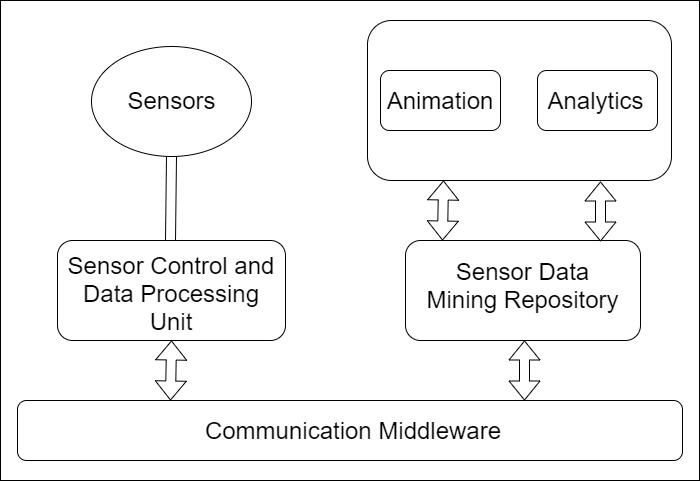
\includegraphics[scale=0.34]{images/fig5.jpg}
  \hspace*{-1.25cm}
  \caption{System Architecture}
  \label{arch}
\end{figure}
\begin{enumerate}
\item Sensors




Sensor networks are new instruments useful to detect the conditions in remote places in the physical world \cite{JD04} in environmental monitoring applications such as pollution monitoring, transportation management, intrusion detection and many more \cite{JLLLNBNR11}. With the help of sensors, it is possible to collect data remotely and collected data can be transferred to the required platform.

There are different sensors available in market which can measure the pollutants and display the value, but the idea here is to select the one which is of low cost and also gives the most accurate values.

 
Sensors will collect data from the environment as per their schedule. Communication module essentially sends the sensor data to mining repository. 


\newpage

 \item {Microcontroller Board}


 
 For simplicity and ease of programming when compared , Arduino Uno can be used which has ATmega328 microcontroller board. Since it is open-source based platform with rich software support, it is a widely used platform for various applications. Arduino supports both digital and analog inputs. As edge computing is preferred in this context, most of the calculation such as measuring gas concentration and computing air quality and air quality health indices are done in Arduino.



 \item {Communication Module}

    For the sensor device to communicate with the IoT software platform  or the software for data analytic and visualization services, I am planning to use ESP8266 WiFi module that has a networkable microcontroller. This module is very compact and has high durability and power saving features. This module transfers the collected data from the microntroller to the data repository in the software environment where the further visualization and data management will be done.
      \end{enumerate}
      
 
 \subsection{Software Architecture}
 
This component is to provide statistical data analysis and visualization through intuitive graphics services to help users to make decisions. Particularly, analytic component is needed to performs statistical functionality and animation component is to display the necessary data to users. I am aiming at a Customizabel Layered Visualization (CLV) which will concentrate the delivering of data for different stakeholders based on their interest. There will be a hierarchical visualization option in which the user themselves can drive through the data and keep on expanding the information as needed.
\newpage

\section{Time-Line}

This chapter gives an overview of the total time required in building a sensor network for pollution monitoring system. It gives an idea of dividing the whole process into different tasks and shows the rough time required to complete each task. The estimated time line for the completion is given below.





\begin{figure}[h!]
  \centering
  \hspace*{-1.40cm}   
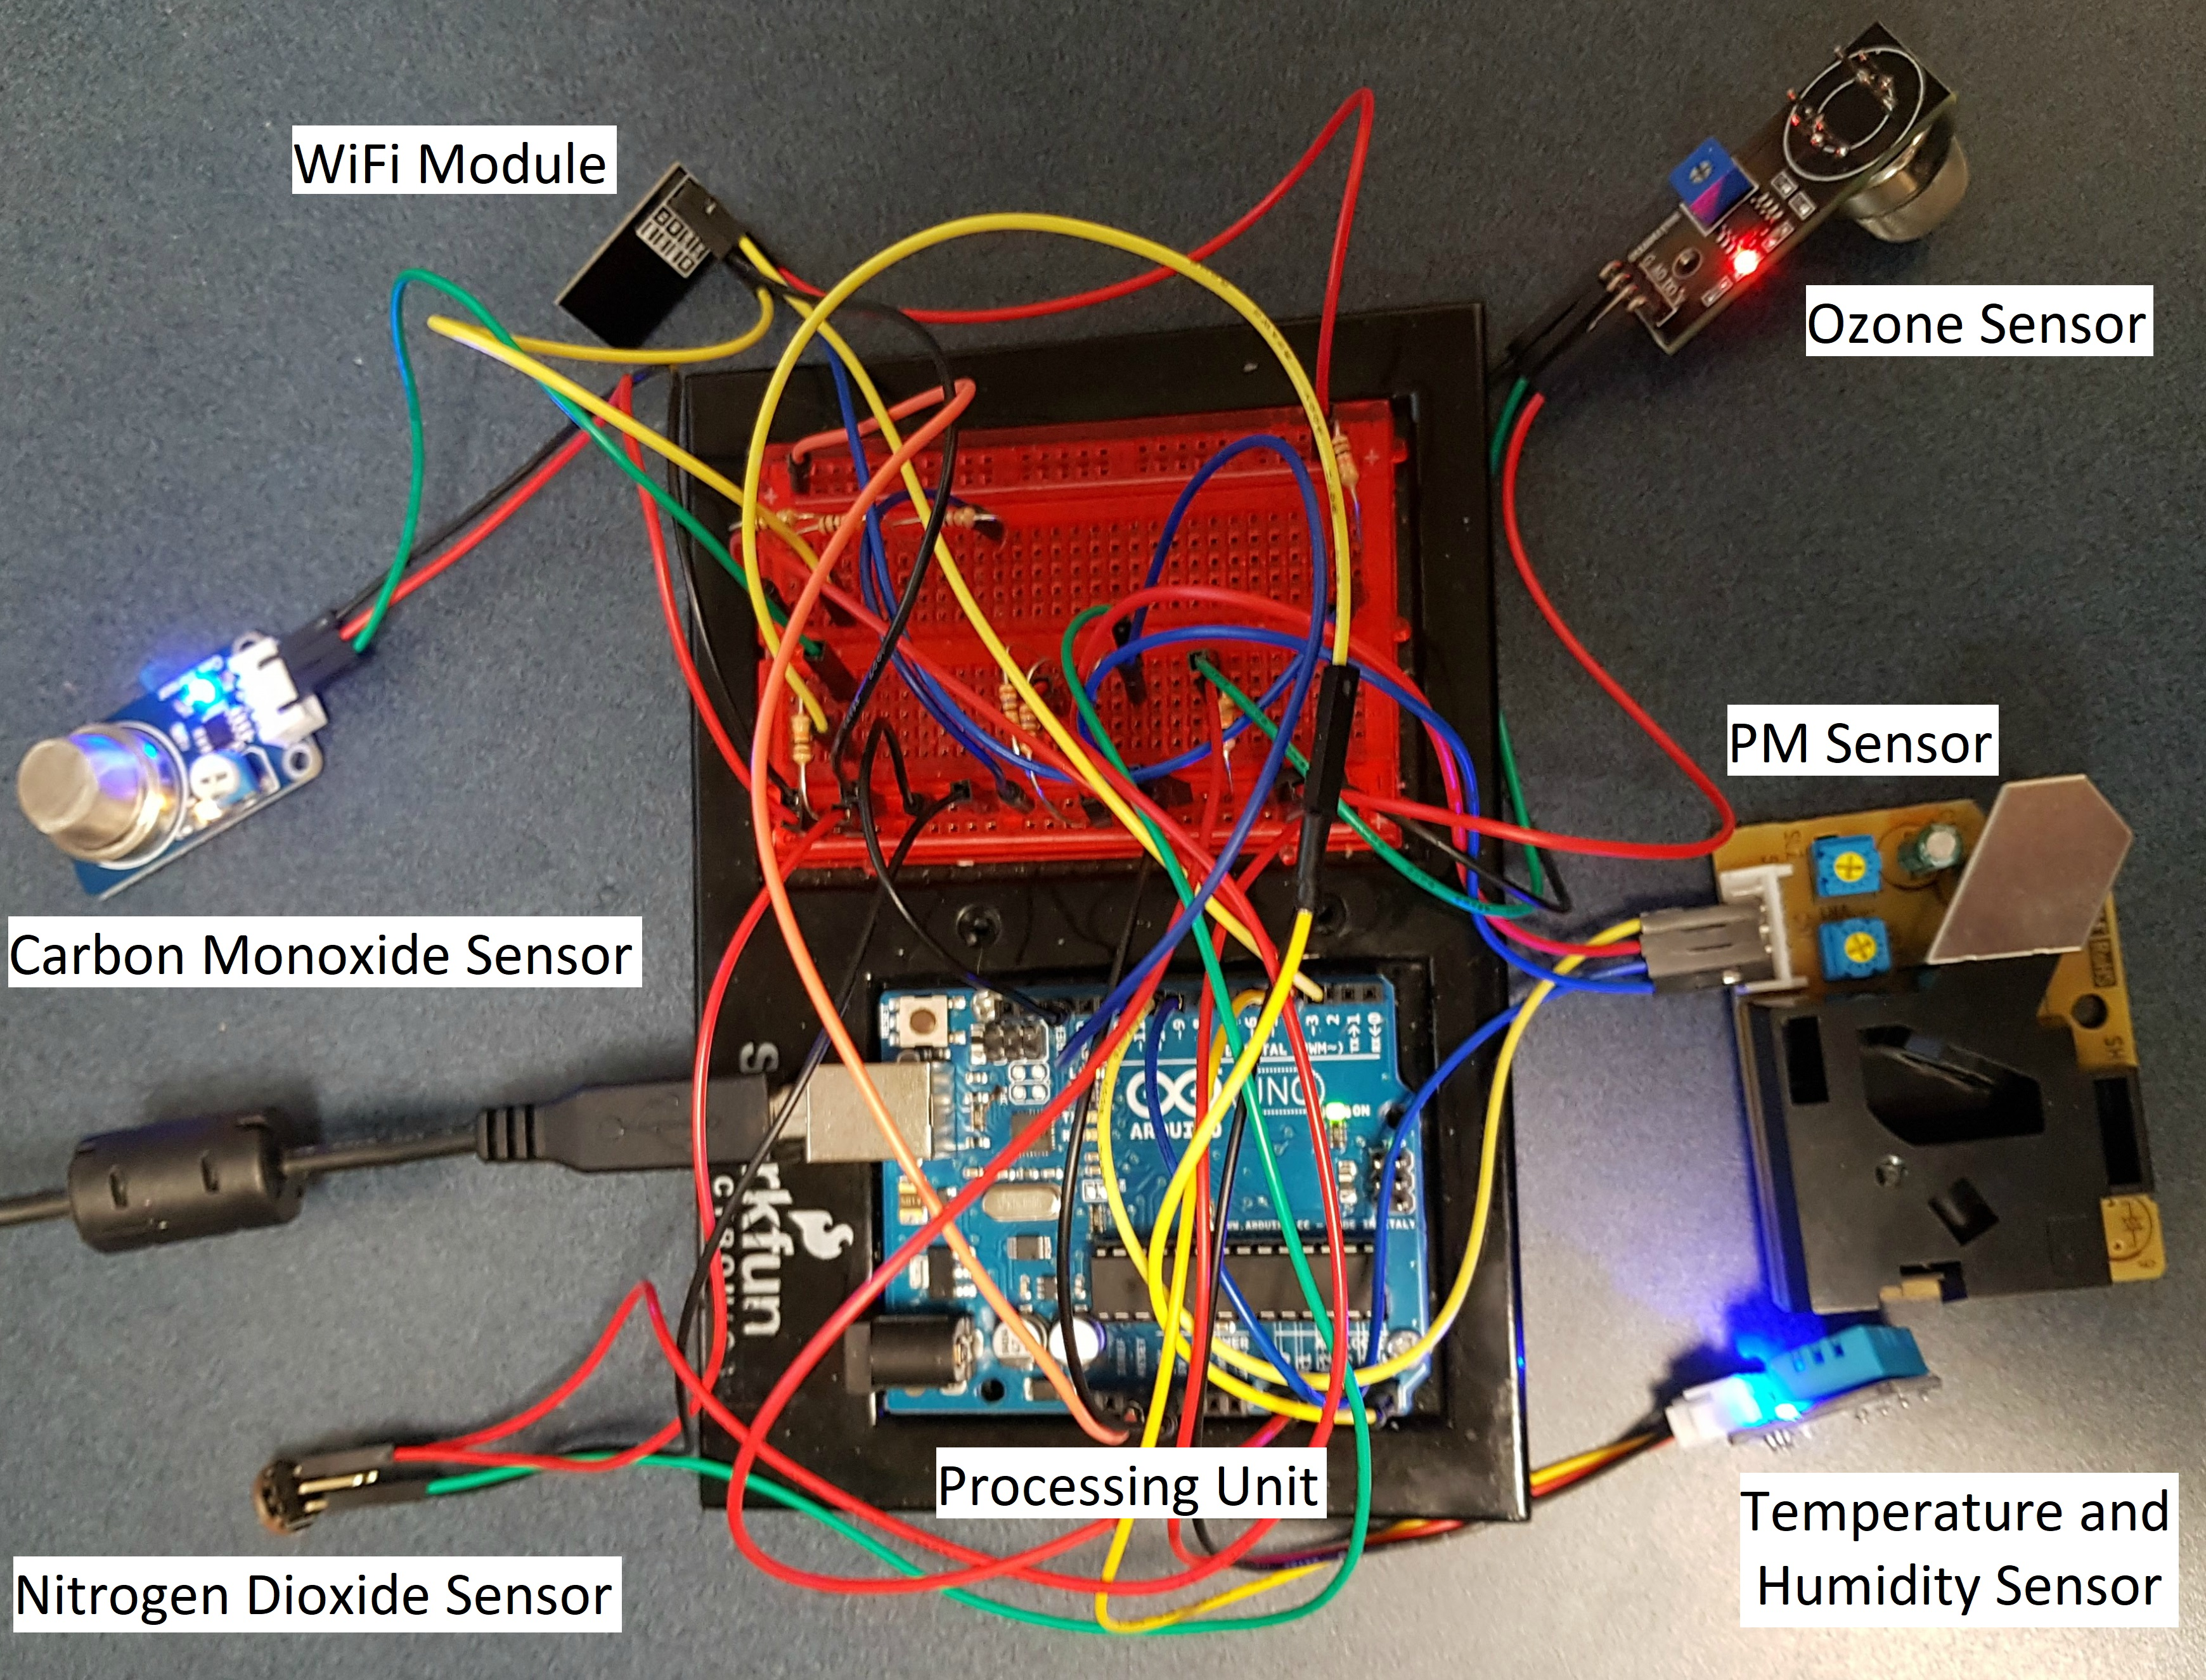
\includegraphics[scale=0.38]{images/fig4.png}
  \hspace*{-1.40cm}
  \caption{Thesis Time-line}
  \label{arch}
\end{figure}
\newpage
\section{Progress}

The hardware part of the system was implemented and the values were collected and represented in an open source platform, Thingspeak, which plotted the value of each pollutant concentration corresponding to a particular time. The implemented system is as shown in figure 3, in which all the sensors are attached to processor. All the sensors were selected carefully based on performance, cost and size so that the system remains compact and portable. For the initial testing of the system the data collected from the hardware was represented in Thingspeak visualization environment itself to understand how the collected data from sensors looks like. Along with the representation of the concentration of pollutant there was also an attempt done in calculating the Air Quality Health Index(AQHI), which was successfully shown along with other graphs. 


\begin{figure}[h!]
  \centering
  \hspace*{-1.25cm}   
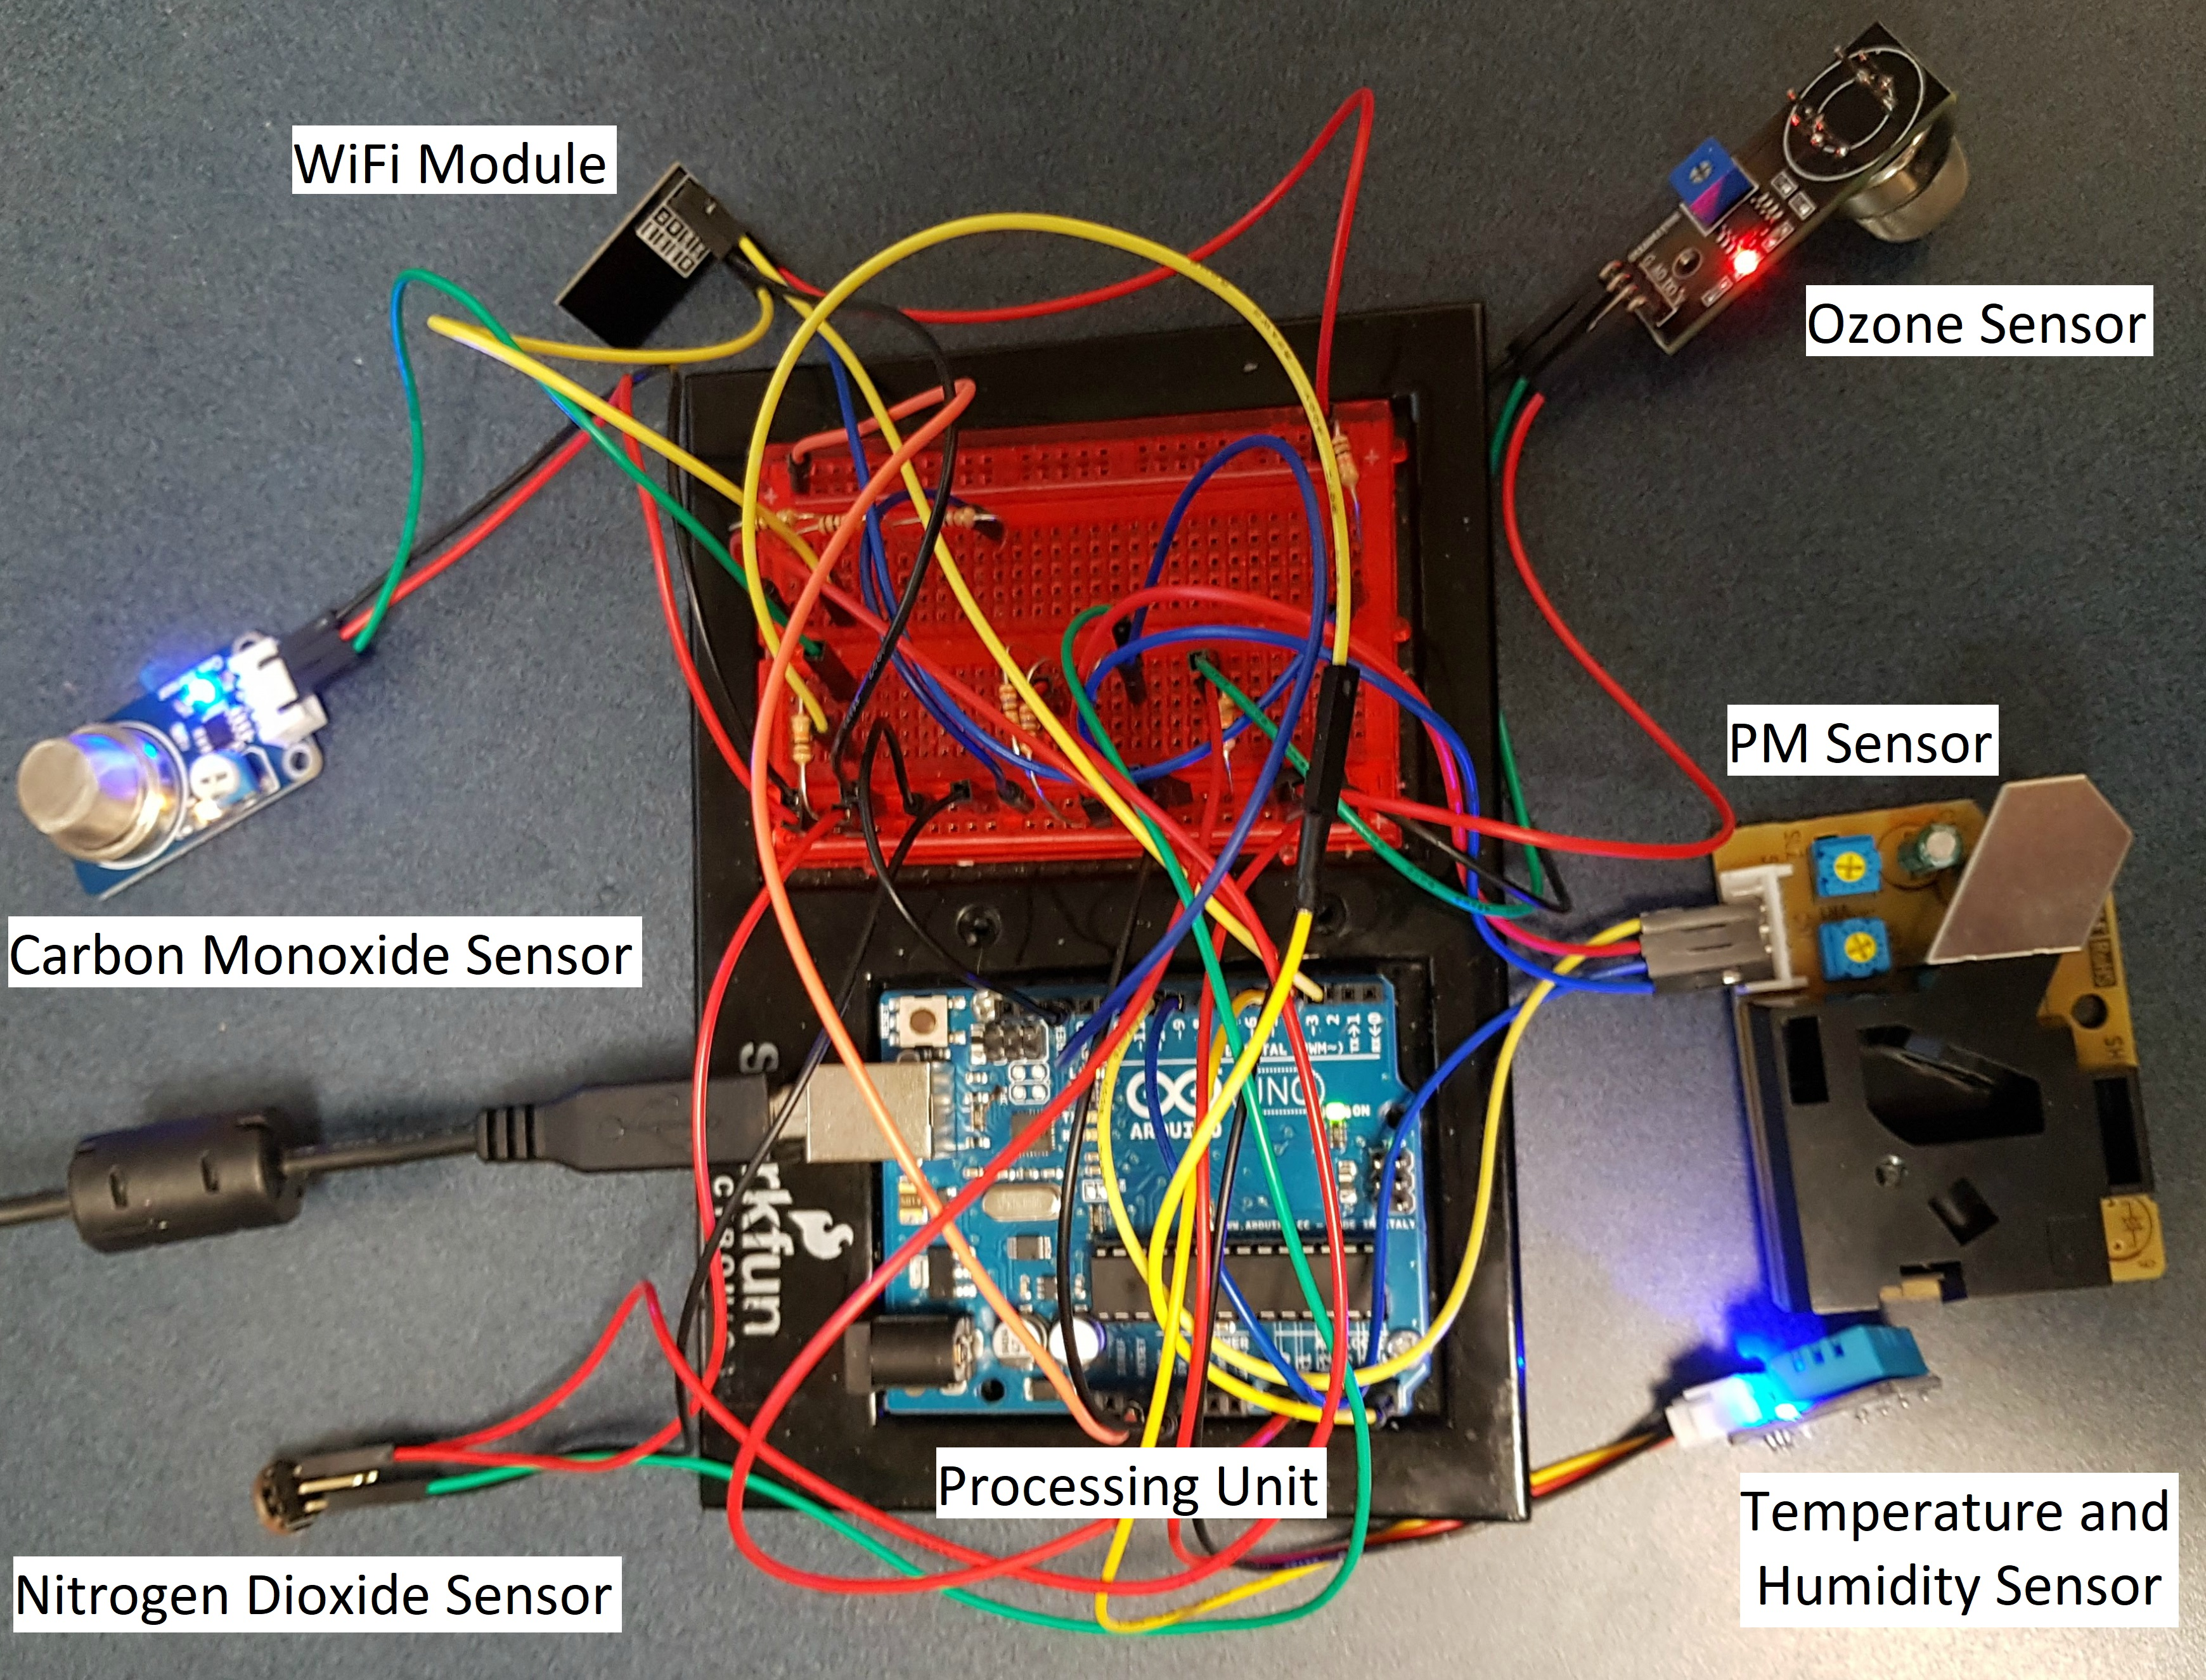
\includegraphics[scale=0.094]{images/fig4.jpg}
  \hspace*{-1.25cm}
  \caption{Hardware System}
  \label{arch}
\end{figure}

The graphs for different pollutants and the index for understanding the effect of pollution is explained in the paper \cite {SA17}. The paper clearly gives an idea about the Thingspeak platform and also about the hardware architecture. There was not much changes made from proposed architecture.




\newpage


\begin{thebibliography}{abrv}



\bibitem{A16} G. Anthes, Open Source Software No Longer Optional, {\it Communications of the ACM}, 59(8):15-17, 2016.

\bibitem{Retal17} M. Rahman, et. al., Adaptive Sensing Using Internet-of-Things with Constrained Communications, {\it ACM/IFIP/USENIX Middleware Conference}, 6 pages, 2017.

\bibitem{Betal17} A. Bagnato, et. al., Designing Swarms of Cyber-Physical Systems: the H2020 CPSwarm Project, 
{\it ACM International Conference on Computing Frontiers}, Invited Paper, 305--312, 2017.

\bibitem{S16} John A. Stankovic, Research Directions for Cyber Physical Systems in Wireless and Mobile Healthcare,
{\it ACM Transactions on Cyber Physical Systems}, 1(1):1:1--12, 2016.

\bibitem{O17} S. F. Ochoa, G. Fortino, and G. D. Fatta, Cyber-physical systems, internet of things and big data (Editorial), {\it Future Generation Computer Systems}, 75:82--84, 2017.

\bibitem{Getal17} G. Guan, et. al., TinyLink: A Holistic System for Rapid Development of IoT Applications,
{\it The 23rd ACM Annual International Conference on Mobile Computing and Networking (MobiCom)}, 2017.

\bibitem {HealthEffectsInstitute2017} Health Effects Institute. State of Global Air 2017. {\it Report}, Health Effects Institute, 2017.

\bibitem{DCRMG17} Joy Dutta, et. al., . Towards Smart City: Sensing Air Quality in City Based on Opportunistic Crowd-sensing. {\it Proceedings of the 18th International Conference on Distributed Computing and Networking}, 42:1--6, 2017. 

\bibitem{YLMLLM15} Wei Ying Yi, et. al., (2015). A Survey of Wireless Sensor Network Based Air Pollution Monitoring Systems. Sensors,  15: , 2015. 

\bibitem{YLL12} James J.Q.Yu, et. al., (2012). Sensor deployment for air pollution monitoring using public transportation system. 2012 {\it IEEE Congress on Evolutionary Computation}, 2:1--7, 2012.  

\bibitem{N15} N. Nannoni,  Message-oriented Middleware for Scalable Data Analytics Architectures.  2015.

\bibitem{KBHG14}
O. Kononenko, O. Baysal, R. Holmes, and M.W. Godfrey. Mining modern repositories with elasticsearch. \textit{In Proceedings of the 11th Working Conference on Mining Software Repositories}. 328-331, May, 2014.

\bibitem{FSK17} M.F.M Firdhous, B.H. Sudantha, P.M. Karunaratne. (2017). IoT enabled proactive indoor air quality monitoring system for sustainable health management. 
{\it Proceedings of the 2nd International Conference on Computing and Communications Technologies (ICCCT)}, 216--221, 2017.

\bibitem{WYM14} Man Sing Wong,Tsan Pong Yip,Esmond Mok,(2014). Development of a Personal Integrated Environmental Monitoring System. {\it Sensors}, 14(11):22065--22081, 2014. 

\bibitem{FXP16} Biyi Fang, et. al.,  AirSense: An intelligent home-based sensing system for indoor air quality analytics. {\it Proceedings of the 2016 ACM International Joint Conference on Pervasive and Ubiquitous Computing}, 109--119, 2016.

\bibitem{H14} Holstius, D. (2014). Monitoring particulate matter with commodity hardware, {\it PhD Thesis}, University of California Berkeley, 2014.

\bibitem{FXPZ16} B.Fang, Q.Xu, T.Park,M.Zhang, (2016). AirSense: An intelligent home-based sensing system for indoor air quality analytics.{\it UbiComp 2016 - Proceedings of the 2016 ACM International Joint Conference on Pervasive and Ubiquitous Computing}

\bibitem {AQI14} Government of India,Ministry of Environment, F.C.C.(2014) National Air Quality Index,58. Retrieved from {\it http:www.indiaenvironmentportal.org.} Air Quality Index.pdf
\bibitem{HR13}  H. Chen,R. Copes,(2013). Review of Air Quality Index and Air Quality Health Index.

\bibitem {JD04}  Elson J., Estrin D, Sensor Networks: A Bridge to the Physical World; Kluwer Academic Publishers: Norwell, MA, USA, 2004; pp. 3-20

\bibitem{Thingspeak} {\it https://thingspeak.com/}

\bibitem{JLLLNBNR11} Jung Y. J., Lee Y. K., Lee D. G., Lee Y., Nittel S., K.Beard, K. H. Ryu(2011). Design of sensor data processing steps in an air pollution monitoring system. Sensors, 11(12), 11235–11250. https://doi.org/10.3390/s111211235.
\bibitem {PXMOC14}  R. Piedrahita,Y.Xiang, N.Masson,J. Ortega, A.Collier,Y. Jiang,L. Shang, (2014). The next generation of low-cost personal air quality sensors for quantitative exposure monitoring. Atmospheric Measurement Techniques, 7(10), 3325–3336. https://doi.org/10.5194/amt-7-3325-2014.

\bibitem {Gov} {\it https://www2.gov.bc.ca/gov/content/environment/air-land-water/air/air-quality/measuring}

\bibitem {SA17} Ashlin.S, Alex.A,  A Cyber-Physical System for Pervasive Air Pollution Monitoring.

\bibitem {SA18} Ashlin.S, Alex.A, Towards Intuitive Visualization of Air Quality Data.

\bibitem {who} {\it http://www.who.int/en/ }

\end{thebibliography}





\end{document}